\section{Design} \label{sec:design}

\begin{figure}[t!] 
     \centering 
     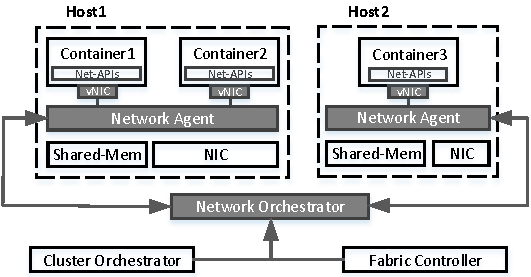
\includegraphics[width=3.5in]{figures/system-arch.pdf} 
    \caption{\label{fig:sysarch} The overall system architecture of~\sysname. Gray boxes are building blocks of~\sysname.} 
\end{figure} 

This section presents the high-level design of \sysname. We introduce
the requirements and concerns in the designs of control-plane, data-plane
and programming interface, and explain what design choices \sysname makes 
and what the reasons are behind these design choices.

\subsection{Overview}

Our goal is to design a completed network solution which can enable containers
to communicate with portability, isolation and high performance at the same time.
This solution has three main components: control-plane, data-plane and programing
abstraction. 

A control-plane handles IP address assignment, routing and keeping global states.
A flexible control-plane is a must for portability and isolation. 
It should permit a container to register its own IP address in the network
from any host, and also should automatically configure and update the routing 
to each container. Different from existing overlay network solutions of 
containers, we also require the control-plane to be able to select 
data-plane mechanisms (e.g. shared-memory, RDMA, TCP/IP, etc.) 
in real-time according to multiple factors, 
such as container locations, hardware capabilities and so on.

A data-plane delivers data from senders to receivers.
Data-plane should always promise the best network performance between 
containers. From measurements (Figure~\ref{XXX}), 
we see that shared-memory has the highest
bandwidth, lowest latency, smallest NIC load and modest CPU load. 
Therefore, shared-memory is favorable to be used as the data-plane 
mechanism between two containers on the same host. 
The data-plane for inter-host communication
depends on the hardware capability. For example, RDMA is preferred to TCP/IP 
if the NICs on the hosts have the support.

A network programming abstraction defines how communication 
performed at the end point side.
For example, the most popular network abstraction for TCP/IP is Socket~\cite{?},
Verbs~\cite{?} is widely accepted for RDMA, and MPI~\cite{?} is a standard for
message-passing in distributed memory and parallel computers. 
We require that
the network programming abstraction of~\sysname must at least have two
properties. First, it facilitates containers to access the network and 
transparently utilize the data-plane mechanisms, and second, it is general 
enough to support existing programming interfaces on top of it for backward 
compatibility. 

The design of~\sysname fully considers the requirements from all these three
components.

\subsection{The architecture of FreeFlow}

Figure~\ref{fig:sysarch} shows the architecture and design choices on each 
components of~\sysname. Network orchestrator is the centralized control-plane
of~\sysname. The local network agent running in each host coordinates
multiple data-plane mechanisms according to the information and 
configurations feed
from the network orchestrator. We choose standard RDMA programming interface --
Verbs API -- as the programming API in the whole solution. Next, we will explains
our design decisions in details. 

\para{Centralized control-plane:} \sysname inherently needs a (conceptually)
centralized control-plane because the IP assignment, routing configuration and 
data-plane mechanism decisions are all computed from the global states of the
container cluster. The network orchestrator of~\sysname maintains three kinds
of global information: the location of each container, the assigned IP of each
container and the capabilities of host NICs.

\para{Integrated Data-plane:} \sysname's local network agent on each host 
obtains the container location information from the network orchestrator. 
It decides to use shared-memory to communicate if two containers are on the
same host, otherwise, it will conduct the communicate going through 
the NIC of its host. Depending on the capability of the NIC, the traffic 
between two hosts can be delivered via RDMA, DPDK or TCP/IP.

\para{RDMA-Verbs based programming abstraction:} We decide to adopt 
RDMA-Verbs API for three reasons. First, in data centers, most of
the applications that have strong desires to high networking performance
are written or are migrating to RDMA based networking abstraction, so that
\sysname can naturally support these applications; Next, Verbs API is a 
widely accepted and used industrial standard; Finally, Verbs API is proven
to be a general and low-level programing interface, and there are already
adaptation layer libraries available to support TCP/IP~\cite{?}
and MPI~\cite{?} on top of Verbs. Given that Verbs API directly talks to
NIC, \sysname provides a virtual RDMA NIC on each container. One virtual NIC
can talk with the process of its container with RDMA protocols and hide
the decisions of local network agent and the actual data-plane mechanism
that is used. 

\subsection{Working flows of FreeFlow}

To support the standard RDMA Verbs API used by containers and realize
communications with the best available data-plane mechanism, \sysname needs
to present a RDMA environment to containers and efficiently supports 
the RDMA semantics with multiple data-plane mechanisms. While RDMA has
four interfaces (e.g. Write, Read, Send and Receive), we use Write as an example
to show how \sysname supports this operation with shared-memory and real RDMA.

Figure XXX (a) shows the working flow of a standard RDMA write from containers'
points of view when they use Verbs API. There are generally three steps in a 
Write operation. 
Step 1: the sender first creates a memory block, puts data in it and passes 
the pointer of this memory block to its NIC;
Step 2: the sender notify its NIC to write the memory block to the receiver's IP.
Step 3: the receiver's NIC will get data from the sender's NIC and copy the 
data into a memory block and pass the pointer of the memory block to the 
receiver.

In \sysname, both the sender and receiver containers have a virtual RDMA NIC.
In Step 1, the sender creates a shared-memory block and write data, and then 
the local network agent will get the pointer of this shared-memory block after the sender passes it to its virtual NIC; In Step 2, after receiving the IP of 
the receiver, the local network agent will check whether the receiver is on
the same host of the sender. If the answer is "Yes", the local network agent will
directly leverage the receiver's virtual NIC to notify it that a memory block 
from RDMA is ready to read with the pointer of the shared-memory block. 
Otherwise, the sender's local network agent will perform an actual RDMA write
with the receiver's local network agent, and the latter will put the received data into a shared-memory and pass it to the receiver container via its virtual NIC.






